\documentclass{article}


\usepackage{PRIMEarxiv}

\usepackage[utf8]{inputenc} % allow utf-8 input
\usepackage[T1]{fontenc}    % use 8-bit T1 fonts
\usepackage{hyperref}       % hyperlinks
\usepackage{url}            % simple URL typesetting
\usepackage{booktabs}       % professional-quality tables
\usepackage{amsfonts}       % blackboard math symbols
\usepackage{nicefrac}       % compact symbols for 1/2, etc.
\usepackage{microtype}      % microtypography
\usepackage{lipsum}
\usepackage{fancyhdr}       % header
\usepackage{graphicx}       % graphics
\graphicspath{{media/}}     % organize your images and other figures under media/ folder

%Header
\pagestyle{fancy}
\thispagestyle{empty}
\rhead{ \textit{ }} 

% Update your Headers here
% \fancyhead[LO]{Rebuttal}
% \fancyhead[RE]{Firstauthor and Secondauthor} % Firstauthor et al. if more than 2 - must use \documentclass[twoside]{article}
\usepackage{pdfpages}
% % 水印
% \usepackage[printwatermark]{xwatermark}
% \usepackage{xcolor}
% \usepackage{background}

% % 定义水印图片
% \newsavebox\mybox
% % \savebox\mybox{\tikz[color=red,opacity=0.3]\node{Example Watermark};}
% % \savebox\mybox{\includegraphics[width=0.05\textwidth]{Project01/LOGO_UST_blue_gold.png}}
% \newwatermark*[
%   allpages,
%   angle=45,
%   scale=6,
%   xpos=-20,
%   ypos=15,
%   opacity=0.99, % 设置水印透明度
% ]{\includegraphics[width=0.5\textwidth,opacity=0.5]{Project01/LOGO_UST_blue_gold.png}}
  
%% Title
\title{REBUTTAL
%%%% Cite as
%%%% Update your official citation here when published 
% \thanks{\textit{\underline{Citation}}: 
% \textbf{Authors. Title. Pages.... DOI:000000/11111.}} 
}

% \author{
%   Author1, Author2 \\
%   Affiliation \\
%   Univ \\
%   City\\
%   \texttt{\{Author1, Author2\}email@email} \\
%   %% examples of more authors
%    \And
%   Author3 \\
%   Affiliation \\
%   Univ \\
%   City\\
%   \texttt{email@email} \\
%   %% \AND
%   %% Coauthor \\
%   %% Affiliation \\
%   %% Address \\
%   %% \texttt{email} \\
%   %% \And
%   %% Coauthor \\
%   %% Affiliation \\
%   %% Address \\
%   %% \texttt{email} \\
%   %% \And
%   %% Coauthor \\
%   %% Affiliation \\
%   %% Address \\
%   %% \texttt{email} \\
% }
\author{%
  Fu Yang \\
  21029346\\
  \texttt{yfubo@connect.ust.hk} \\
  \And
  Luo Yuqing \\
  20582315\\
  \texttt{yluobb@connect.ust.hk} \\
  \AND
  Wang Jinyuan \\
  21028990\\
  \texttt{jwangiy@connect.ust.hk} \\
  \And
  Wang Tong \\
  20905737\\
  \texttt{twangce@connect.hk} \\
}


\begin{document}
\maketitle


\begin{abstract}
This rebuttal is for the peer reviews from four classmates about our MAFS6010Z's first homework which is a home-credit-default-risk kaggle contest. We summarized their peer reviews into four opinions and gave our reasons to refute them. Our model advocates using mature relevant theories under limited time and limited computing resources, and quickly and accurately putting forward our own algorithms for the problem without plagiarizing existing external solutions.
\end{abstract}

\section{Opinions}
\textbf{Opinion1:} 
\textit{It would be helpful to address outlier handling, particularly for variables like DAYS\_BIRTH and DAYS\_EMPLOYED, which are highly correlated with the target variable and contain internal outliers.}\ref{review1}

\textbf{Response1:} 
\begin{itemize}
    \item Highly correlated with the target variable: It depends on the actual situations. It is common sense that the risk of default is related to the age. It's reasonable.
    \item Outliers: It is true that outliers would cause model instability. But on the other hand, outliers also contains some information. Those applications with false data may be fraud. And tree model could separate them.
\end{itemize}

\noindent\rule[0.5ex]{16cm}{1pt}

\textbf{Opinion2:} 
\textit{It is worth noting that LabelEncoder may not be suitable for non-numeric variables without a clear ordinal relationship, and considering alternative methods like OneHotEncoder would be more appropriate.}\ref{review1}

\textbf{Response2:}
Trees can easily handle qualitative predictors without the need to create dummy variables. You could check lecture04\_tree, page41 from MAFS6010z.\cite{yaoyuan1}

\noindent\rule[0.5ex]{16cm}{1pt}

\textbf{Opinion3:} 
\textit{Additionally, providing more clarity on the differences and considerations between XGBoost and LightGBM models, including their support for GPU training and multi-threading, would enhance the analysis. It is worth noting that XGBoost also supports multi-threading and GPU.}\ref{review1}


\textbf{Response3:}
The classmate did not read our thesis and code carefully. We did not say XGboost didn't support GPU and multi\-threading. We tested the calculating speed difference using GPU and not using GPU.\cite{mitchell2018xgboost}

\noindent\rule[0.5ex]{16cm}{1pt}

\textbf{Opinion4:} 
\textit{ While the report focuses on a single model, LightGBM, it could be beneficial to explore ensemble learning with multiple models to reduce prediction variance}\ref{review1}

\textbf{Response4:}
The single model problem they raised is simple. Based on the industry experiences, we know tree model fits this kind of problems.\cite{gupta2017analysis} Default risk prediction models usually need to deal with a large number of features and samples, and LightGBM has an efficient training and prediction speed, which can handle large-scale datasets. Secondly, default risk prediction models need to consider the interaction between different features, and LightGBM uses a histogram-based decision tree algorithm, which can effectively capture the nonlinear relationships and interactions between features.

\noindent\rule[0.5ex]{16cm}{1pt}

\textbf{Opinion5:} 
\textit{there is a typo on page 4 where the report says \'im value\' when it probably should be \'importance value\'}\ref{review2}

\textbf{Response5:}
Regarding the typo on page 4, it was just an abbreviation and not a significant issue.

\noindent\rule[0.5ex]{16cm}{1pt}

\textbf{Opinion6:} 
\textit{the feature engineering part was done completely by Featuretools, which performed automatically without any economic logic. I believe constructing some features based on domain knowledge would boost the model. }\ref{review2}

\textbf{Response6:}
The use of Featuretools for feature engineering was a deliberate choice.\cite{schreck2018ai} This framework is proficient at converting time and relational datasets into feature matrices for machine learning. It provides a convenient and efficient way to perform transformations across multiple tables with minimal code. Featuretools also offers the flexibility to create custom primitives, and its performance optimizations make it a powerful complement to pandas. Therefore, while we agree that domain knowledge can enhance feature engineering, we believe that the automated Featuretools approach was suitable for this task.

\noindent\rule[0.5ex]{16cm}{1pt}

 \textbf{Opinion7:} 
\textit{a thorough data exploration analysis should include more information about the data, such as important tendency, variability, distribution of variables, as well as correlation and relationships within the dataset.}\ref{review2}

\textbf{Response7:}
We understand that the data exploration part may seem insufficient, but even if these analyses are done for each variable, nothing will be done subsequently, so there is no need to do these analyses; As for the correlation and relationships within the dataset, we used a tree model, which is not sensitive to such high collinearity\cite{TOMASCHEK2018249}, so we did not find it necessary to include this analysis.

\noindent\rule[0.5ex]{16cm}{1pt}

\textbf{Opinion8:} 
\textit{the hyperparameter tuning part is not quite convincing. All the best parameters that the
team got were the upper bounds of the ranges that they had set. In this case, I think
it’s better to raise the upper bounds and find if there’re better parameters for the
model.}\ref{review2}

\textbf{Response8:}
Regarding the hyperparameter tuning, The upper bounds of the hyperparameters were indeed reached in our tuning process. However, this was not due to an oversight but rather a consideration of computational resources. We appreciate your suggestion to raise the upper bounds, and we will consider this in future projects once we have more computational resources at our disposal.

\noindent\rule[0.5ex]{16cm}{1pt}

\textbf{Opinion9:} 
\textit{there isn’t any conclusion for the result. For example, deep analysis on feature importance and summary on which attributes of a client can be highly correlated with loan default probability}\ref{review2}

\textbf{Response9:}
We agree that a more detailed conclusion could provide additional insights. However, the scope of this report did not include a deep analysis of feature importance or a summary of attributes correlated with loan default probability. We will consider your suggestion when defining the scope for future reports.

\noindent\rule[0.5ex]{16cm}{1pt}

\textbf{Opinion10:} 
\textit{While the report mentions the imbalance in the target variable, a more in-depth discussion could benefit from how this was addressed during modeling}\ref{review3}

\textbf{Response10:}
As for imbalance discussion, to solve the imbalance problem, we use parameter, class\_weight='balanced', in Lightgbm algorithm. LightGBM automatically adjusts the weight of each class based on the number of samples in each class in the training data, so that each class contributes equally to the model training. It mainly changed the loss function which would affect the gradient.

For example, the model has $n_1$ positive samples and $n_2$ negative samples, the weights are $w_1$ and $w_2$, we have:

$$n_1\times w_1 = n_2 \times w_2$$




% keywords can be removed
% \keywords{First keyword \and Second keyword \and More}


% \section{Introduction}
% \lipsum[2]
% \lipsum[3]


% \section{Headings: first level}
% \label{sec:headings}

% \lipsum[4] See Section \ref{sec:headings}.

% \subsection{Headings: second level}
% \lipsum[5]
% \begin{equation}
% \xi _{ij}(t)=P(x_{t}=i,x_{t+1}=j|y,v,w;\theta)= {\frac {\alpha _{i}(t)a^{w_t}_{ij}\beta _{j}(t+1)b^{v_{t+1}}_{j}(y_{t+1})}{\sum _{i=1}^{N} \sum _{j=1}^{N} \alpha _{i}(t)a^{w_t}_{ij}\beta _{j}(t+1)b^{v_{t+1}}_{j}(y_{t+1})}}
% \end{equation}

% \subsubsection{Headings: third level}
% \lipsum[6]

% \paragraph{Paragraph}
% \lipsum[7]

% \section{Examples of citations, figures, tables, references}
% \label{sec:others}
% \lipsum[8] \cite{kour2014real,kour2014fast} and see \cite{hadash2018estimate}.

% The documentation for \verb+natbib+ may be found at
% \begin{center}
%   \url{http://mirrors.ctan.org/macros/latex/contrib/natbib/natnotes.pdf}
% \end{center}
% Of note is the command \verb+\citet+, which produces citations
% appropriate for use in inline text.  For example,
% \begin{verbatim}
%    \citet{hasselmo} investigated\dots
% \end{verbatim}
% produces
% \begin{quote}
%   Hasselmo, et al.\ (1995) investigated\dots
% \end{quote}

% \begin{center}
%   \url{https://www.ctan.org/pkg/booktabs}
% \end{center}


% \subsection{Figures}
% \lipsum[10] 
% See Figure \ref{fig:fig1}. Here is how you add footnotes. \footnote{Sample of the first footnote.}
% \lipsum[11] 

% \begin{figure}
%   \centering
%   \fbox{\rule[-.5cm]{4cm}{4cm} \rule[-.5cm]{4cm}{0cm}}
%   \caption{Sample figure caption.}
%   \label{fig:fig1}
% \end{figure}

% \subsection{Tables}
% \lipsum[12]
% See awesome Table~\ref{tab:table}.

% \begin{table}
%  \caption{Sample table title}
%   \centering
%   \begin{tabular}{lll}
%     \toprule
%     \multicolumn{2}{c}{Part}                   \\
%     \cmidrule(r){1-2}
%     Name     & Description     & Size ($\mu$m) \\
%     \midrule
%     Dendrite & Input terminal  & $\sim$100     \\
%     Axon     & Output terminal & $\sim$10      \\
%     Soma     & Cell body       & up to $10^6$  \\
%     \bottomrule
%   \end{tabular}
%   \label{tab:table}
% \end{table}

% \subsection{Lists}
% \begin{itemize}
% \item Lorem ipsum dolor sit amet
% \item consectetur adipiscing elit. 
% \item Aliquam dignissim blandit est, in dictum tortor gravida eget. In ac rutrum magna.
% \end{itemize}


% \section{Conclusion}
% Your conclusion here

% \section*{Acknowledgments}
% This was was supported in part by......

%Bibliography
\bibliographystyle{unsrt}  
\bibliography{references}  

\newpage
\textbf{Peer Review1}\label{review1}
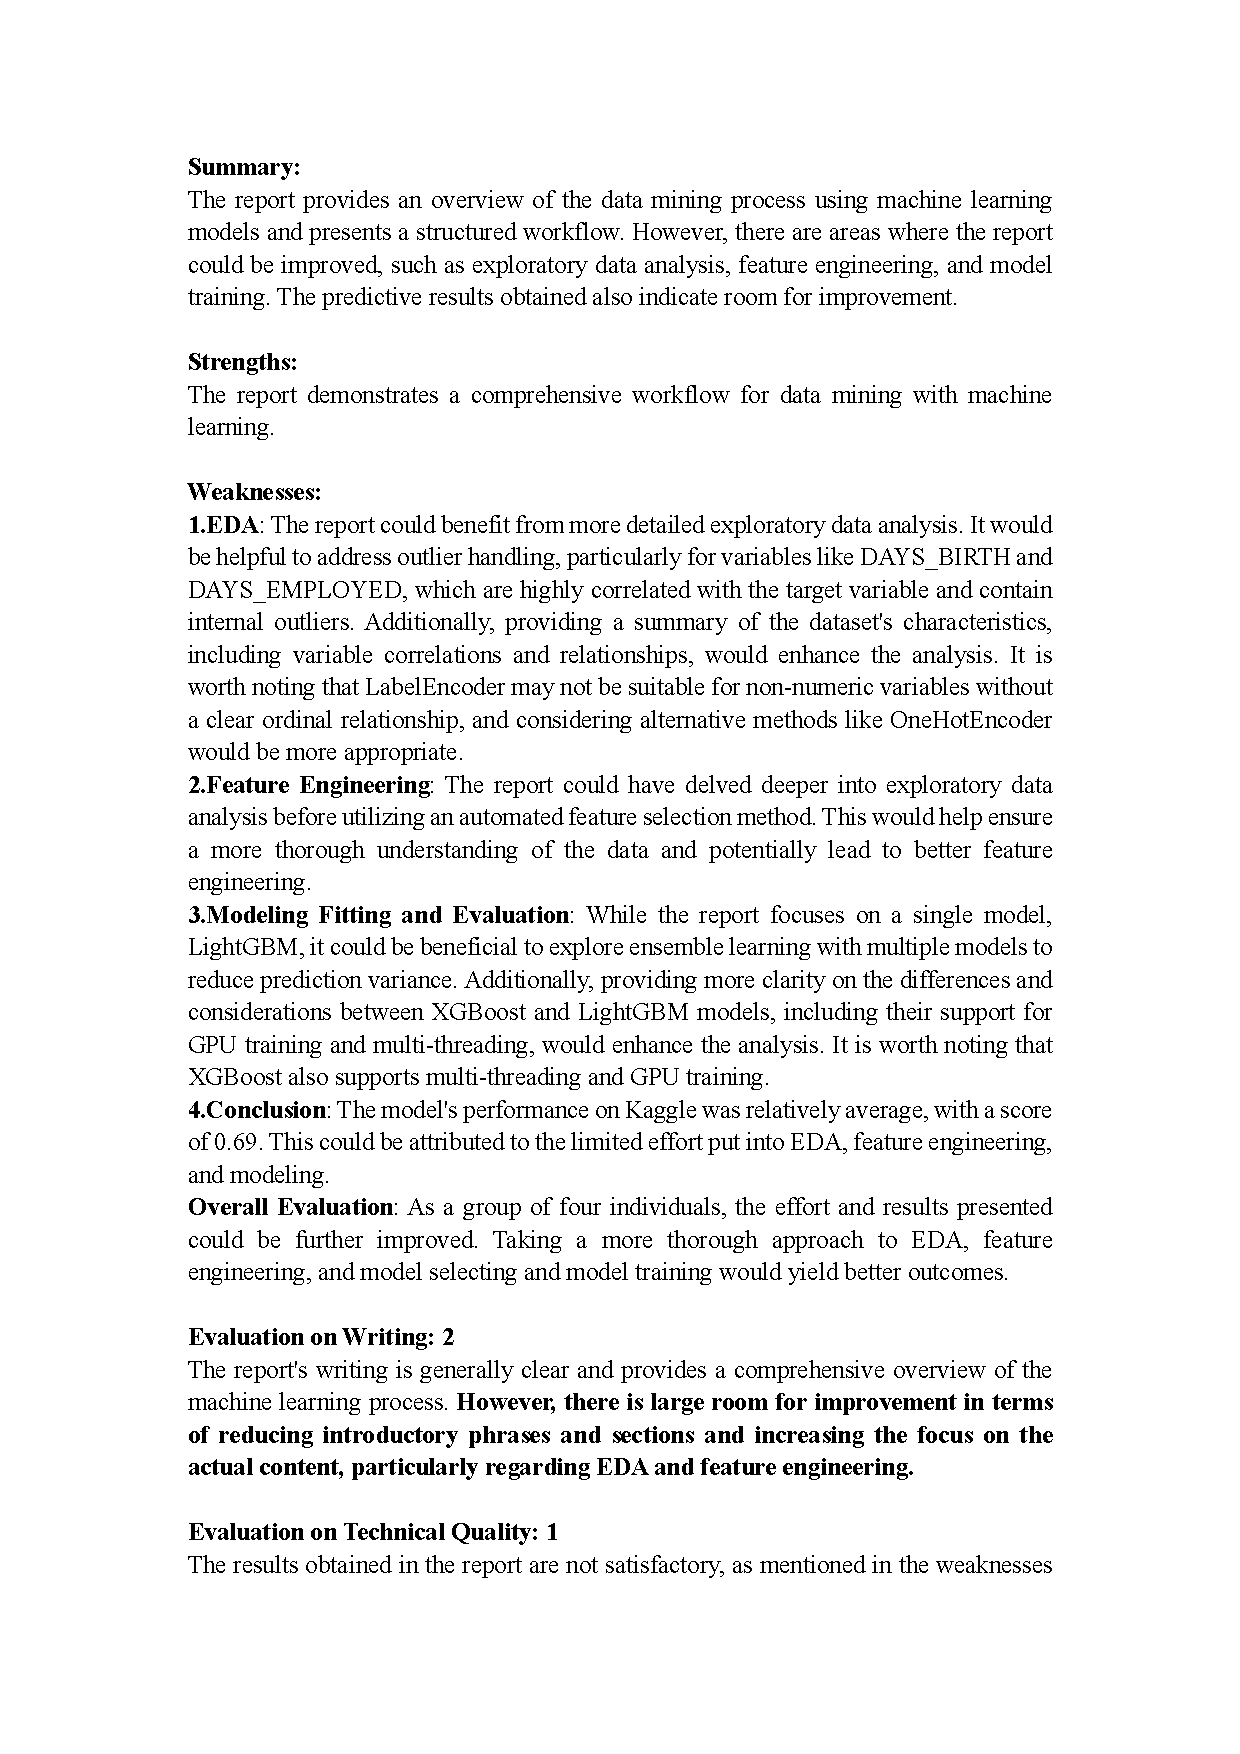
\includepdf{./peer_review1.pdf}

\newpage
\textbf{Peer Review2}\label{review2}
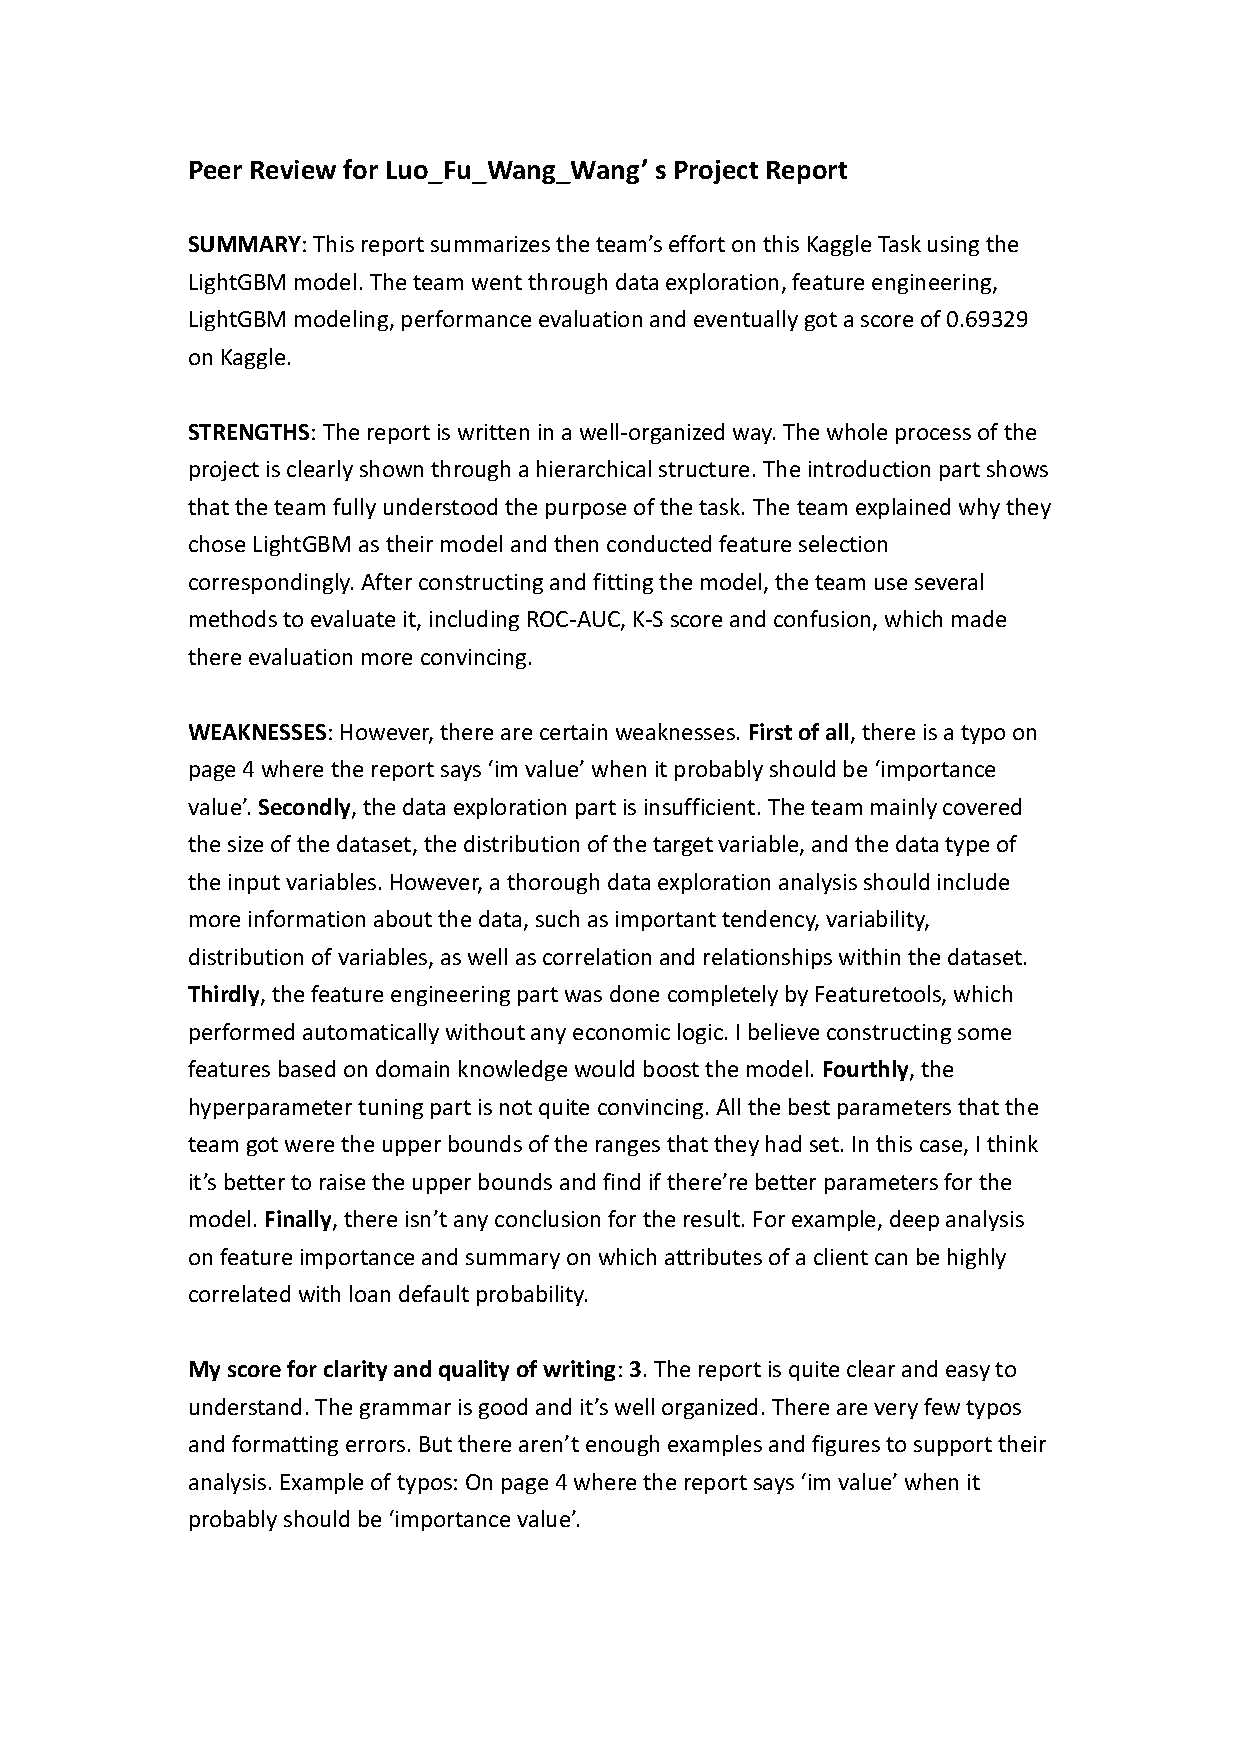
\includepdf{./peer_review2.pdf}

\newpage
\textbf{Peer Review3}\label{review3}
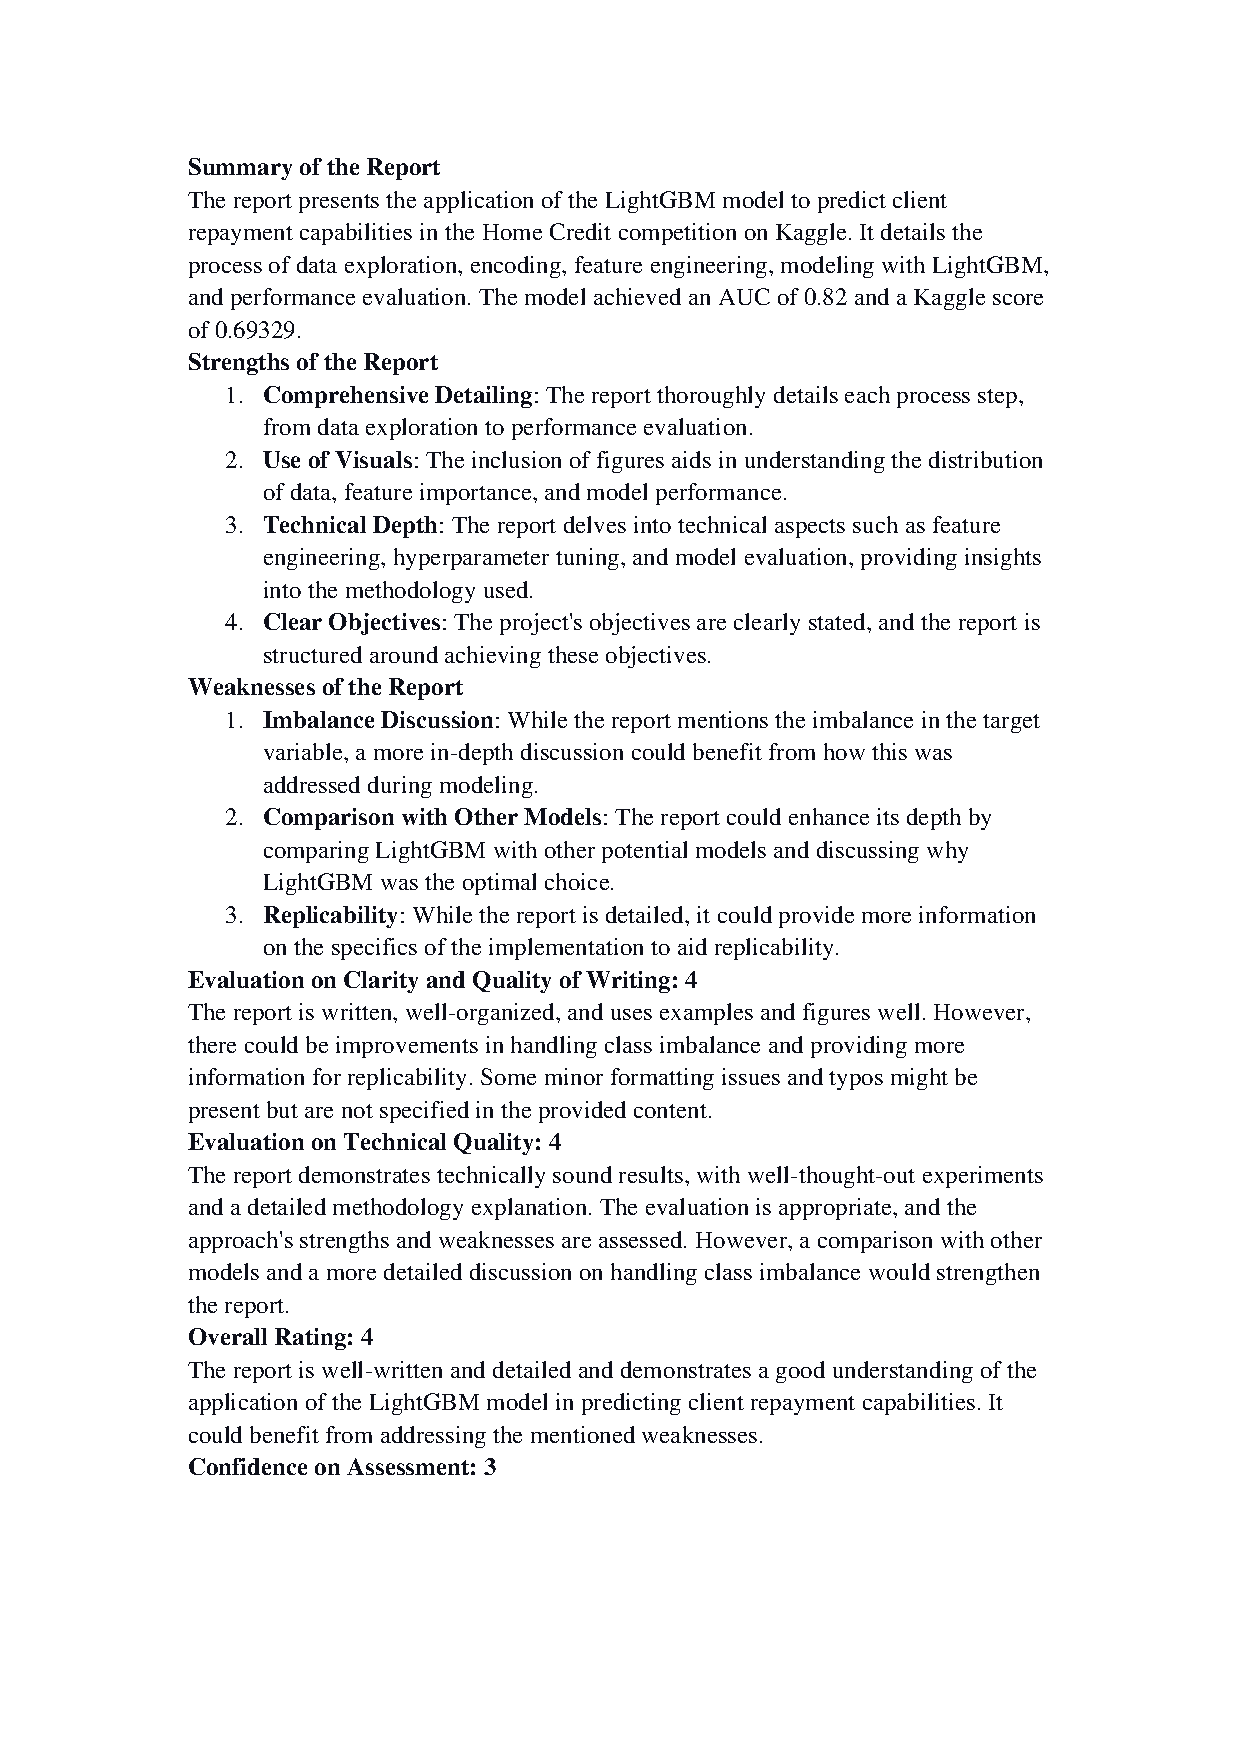
\includepdf{./peer_review3.pdf}

\newpage
\textbf{Peer Review4}\label{review4}
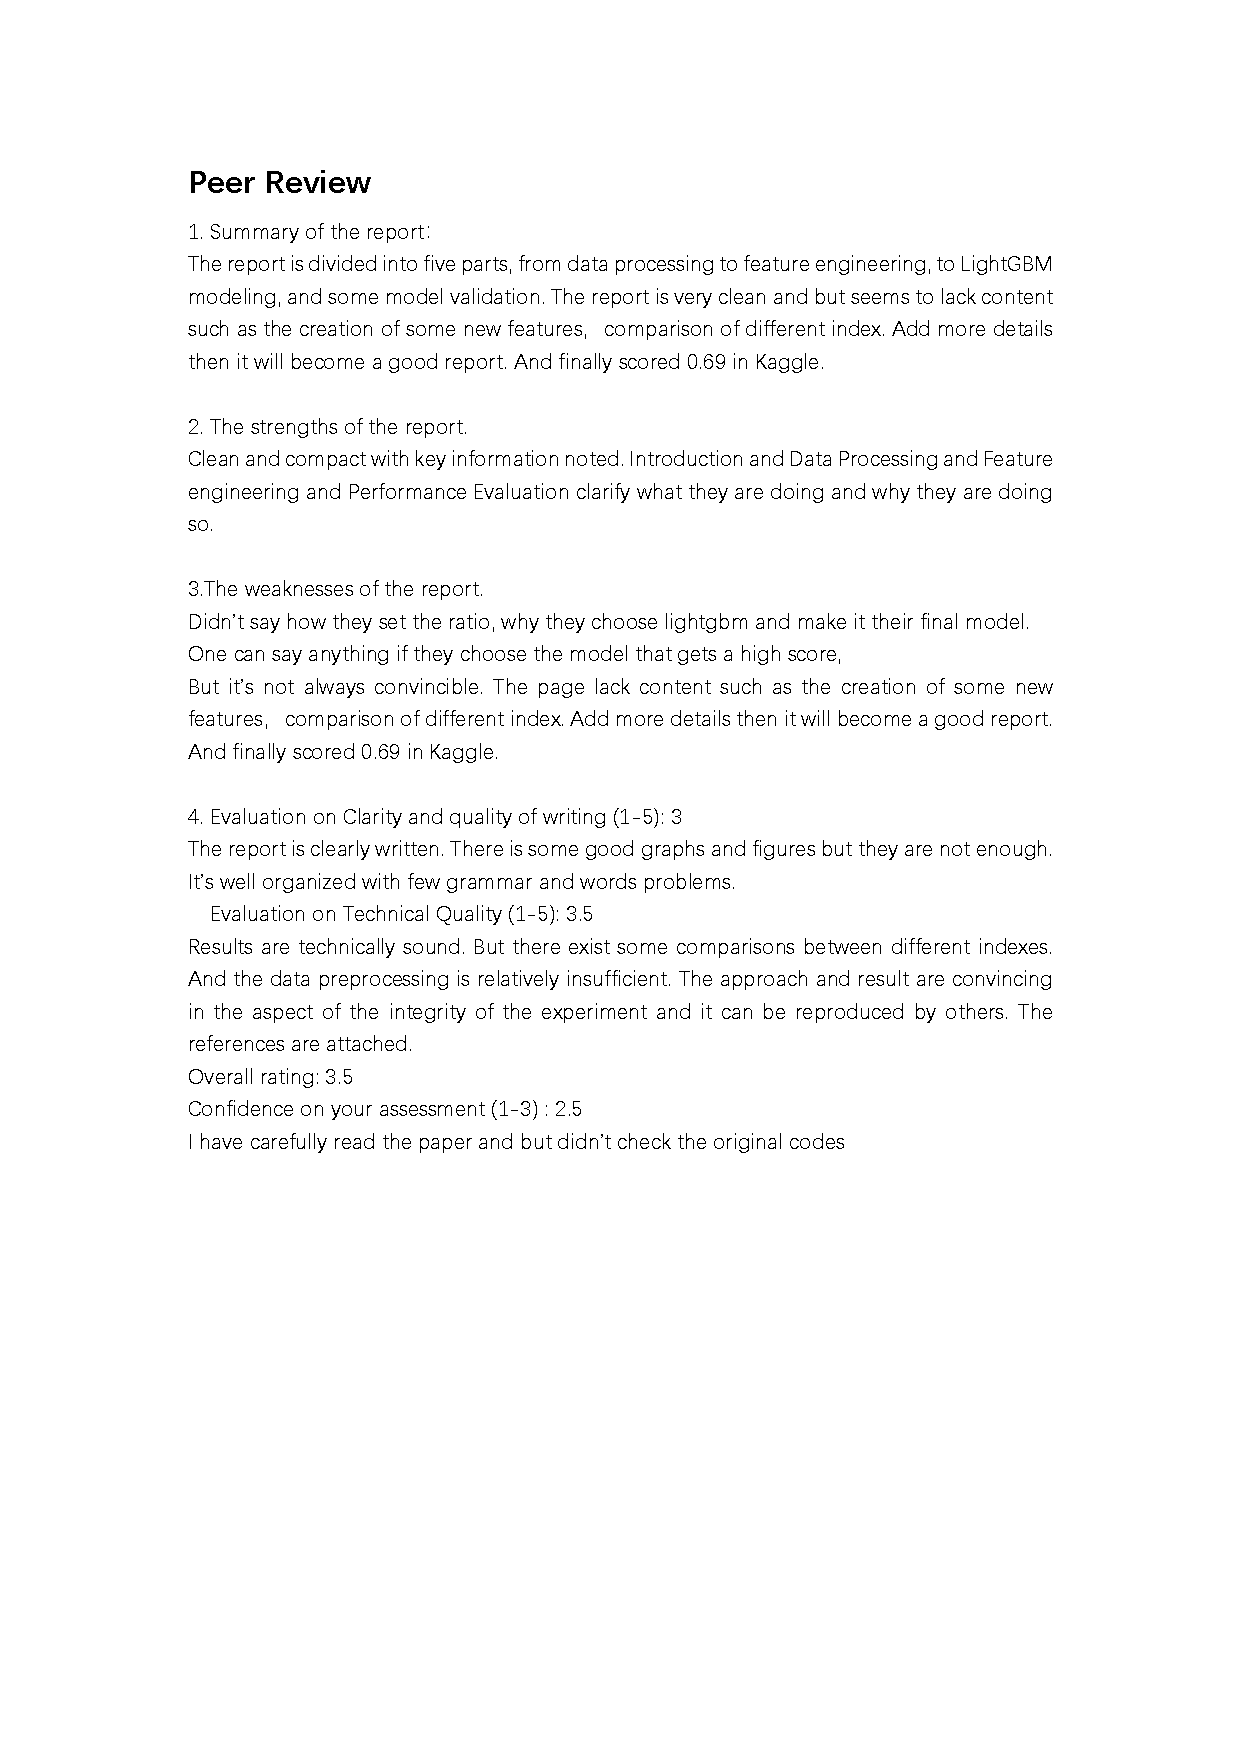
\includepdf{./peer_review4.pdf}

\end{document}
